\subsection{Infrastructure}
\label{subsec:infrastructure}

\subsubsection{Accelerating Rollout Generation with Multi-Token Prediction}

During RL and MOPD, we train using a one-step off-policy asynchronous RL setup, so rollout generation is overlapped with the policy update, and the step time is bounded by whichever stage is slower.
In our setting, the slower stage is typically rollout generation, whose time is in turn dominated by a small fraction of straggler generations that run substantially longer than the rest of the batch.
In order to accelerate rollout generation, we use speculative decoding with Multi-Token Prediction (MTP).
At each decoding iteration, the MTP head is applied recurrently to propose $k$ candidate tokens, which the base model verifies in a single forward pass.
Accepted tokens are committed without additional sequential decoding steps.


\begin{figure}[!ht]
    \centering
    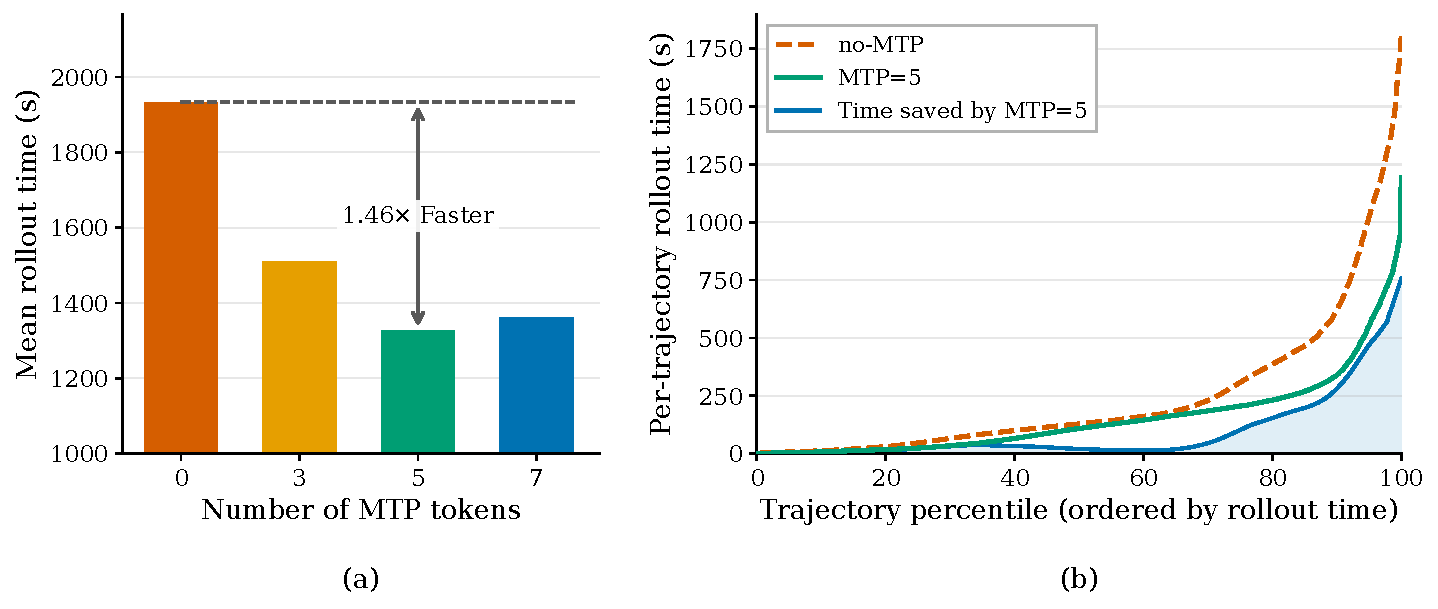
\includegraphics[width=0.9\linewidth]{figures/mtp_rollouts.pdf}
    \vspace{-0.5em}
    \caption{(a) Mean per-step rollout-generation time during RLVR training vs.\ number of MTP tokens $k$. $k{=}5$ gives a $1.46\times$ speedup over the $k{=}0$ (no MTP) dashed baseline. (b) Per-trajectory rollout time for a representative RLVR rollout step, $k{=}5$ vs.\ no-MTP (trajectories ordered by rollout time), and the time saved by MTP. The benefit is concentrated in the long-tail (slowest) generations.}
    \label{fig:mtp_rollouts}
    \vspace{-0.5em}
\end{figure}



To find the best $k$, we sweep $k \in \{0, 3, 5, 7\}$, where $k{=}0$ is the standard no-MTP baseline.
As shown in Figure~\ref{fig:mtp_rollouts}(a), enabling MTP speeds up rollout generation, with $k{=}5$ giving the largest gain at $1.46\times$ over the baseline.
Examining the per-trajectory rollout times for a representative rollout step (Figure~\ref{fig:mtp_rollouts}(b)), we find MTP is particularly beneficial for the long-tail (slowest) generations.
We attribute this to a combination of factors: these long generations emit many more tokens, and they decode toward the end of the batch at lower concurrency, where speculative decoding tends to be most effective.


\subsubsection{Scaling RL Infrastructure}
\noindent Our production cluster is deployed on NVIDIA GB200 nodes with Slurm orchestration and co-located CPUs for sandbox execution. The observed RL software failure breakdown is shown in Table~\ref{tab:failure-attribution}.
\begin{table}[!ht]
\centering
\begin{tabular}{lr}
\hline
\textbf{Failure Category} & \textbf{\%} \\
\hline
Generation engine failures / timeouts & 56 \\
Sandbox / tool calling & 36 \\
Other Software issues & 8 \\
\hline
\end{tabular}
\caption{Failure attribution. Generation and sandbox/tool calling failures account for $\sim$92\% of the failures.}
\label{tab:failure-attribution}
\end{table}

\begin{table}[!ht]
\centering
\begin{tabular}{lcc}
\toprule
\textbf{Issue} & \textbf{Before} & \textbf{After} \\
\midrule
Ray GCS startup           & 30+ min          & 10 min \\
Checkpoint blocking       & 60 sec              & {$<$1 sec} \\
Cold init (JIT)           & 38.8 min         & 0.4 min \\
Multi-node vLLM startup   & 25 min           & 9.5 min \\
Container extraction      & 2--3 min (with cascading failures) & $\sim$0s (warm) \\
\bottomrule
\end{tabular}
\caption{Summary of key infrastructure optimizations and their impact.}
\label{tab:improvements}
\end{table}

Achieving high resiliency required a sustained engineering effort through systematic instrumentation and optimizations, which we subsequently review in detail. 

\subsubsection*{Ray GCS Scalability and Slurm Launch Overheads}
The NeMo-RL job is heterogeneous, it must launch different roles (training workers, vLLM generation workers, gym workers, and judge workers), each with different resource requirements,  across different node subsets. At the start of post-training, our RL launch script issued multiple, separate \texttt{srun} invocations per node to assign each node its role, start its processes, and monitor progress. Each \texttt{srun} is an RPC to the Slurm controller daemon (\texttt{slurmctld}), which must process them serially. At scale, this meant hundreds of serial RPCs queued against \texttt{slurmctld}, a pattern that scaled $O(n)$ with the node count and quickly became a scaling bottleneck. Restructuring to a single multi-node \texttt{srun} reduced Slurm controller interactions to $O(1)$. Together, startup cost dropped from over 30 minutes to 10 minutes..

Additionally, the RL job creates a massive number of Ray actors simultaneously across policy, generation, and environment workers. At 3K+ GPU scale, Ray's single-threaded Global Control Service (GCS) was overwhelmed by actor registrations, causing long startups (25-49 minutes) and thundering-herd startup failures. We eliminated 40\% of actor registrations by converting short-lived actors to tasks, pooling initialization actors per node, and applied aggressive GCS tuning. Anyscale resolved the GCS scalability regressions with the fixes shipped in the Ray 2.55 public release.

\subsubsection*{Topology-Aware NVLink Domain Placement}

On GB200 NVL72, the NVLink domain spans an entire rack (72 GPUs across 18 nodes). Without
topology awareness during worker placement, Megatron's Expert Parallelism (EP) groups can span multiple
racks, forcing MoE all-to-all communication over InfiniBand instead of NVLink.

NeMo RL had no concept of NVLink domains: Ray node IDs are random UUIDs with no
topological relation, and Megatron trusts the rank order it receives. If the
framework assigns ranks without NVLink domain awareness, EP groups will silently
span racks. The fix was to make rank assignment domain-aware and ensure all GPUs
within an EP group are co-located on the same rack. Note that inter-rack ordering
is not a concern here, as our DP size does not require exploiting cross-rack rail
optimizations.

The fix was threefold. First, at container startup (before \texttt{ray start}),
\texttt{ray.sub} generates and sources a probe script that parses the NVLink fabric
\texttt{ClusterUUID} from \texttt{nvidia-smi -q} -- a hex string identical for all
GPUs in the same NVLink domain -- and registers it as a Ray custom resource
(\texttt{nvlink\_domain\_<ClusterUUID>}), giving the scheduler rack-membership
information it previously lacked. The same probe derives a topology rank
(\texttt{topo\_rank}) from \texttt{SLURM\_TOPOLOGY\_ADDR}, falling back to
\texttt{SLURM\_PROCID} or hostname digits. Second, inside NeMo RL's
\texttt{RayVirtualCluster}, bundle indices are sorted by a
$(\texttt{domain\_min\_topo\_rank},\ \texttt{topo\_rank},\ \texttt{gpu\_id})$
composite key, ordering NVLink domains by their minimum topology rank and nodes
within each domain by physical position, so that EP groups remain within a single
NVLink domain. When \texttt{segment\_size} is set, bundles from domains that cannot
contribute a complete segment are discarded. The sorted order drives per-worker
\texttt{RANK} and \texttt{CUDA\_VISIBLE\_DEVICES} assignment, and Megatron runs with
\texttt{external\_gpu\_device\_mapping=True} so it trusts Ray's GPU pinning rather
than re-deriving device placement. Third, the \texttt{topo\_rank} (from
\texttt{SLURM\_TOPOLOGY\_ADDR}) corrects the scrambled Slurm block ordering, with
\texttt{ray.sub} additionally applying a deterministic hostname sort before
Ray head-node assignment.

With these changes, training and generation actors are co-located in the same
NVLink domain, and EP all-to-all traffic stays on NVLink instead of falling back to InfiniBand.

This optimization delivered a \textbf{20\% end-to-end throughput improvement} on GB200.


\subsubsection*{NUMA Binding for Policy and vLLM Workers}

On GB200 NVL72, each compute tray contains a Grace CPU with two sockets and multiple NUMA 
nodes. GPUs are physically affiliated with specific CPU sockets: GPUs~0 and~1 map to NUMA 
node~0, while GPUs~2 and~3 map to NUMA node~1. Without explicit NUMA binding, Ray worker 
processes, both Megatron policy workers and vLLM generation workers, could be scheduled on 
CPU cores belonging to the remote socket relative to their assigned GPUs. On 
Grace-Blackwell, the NVLink-C2C interconnect between Grace CPU and Blackwell GPU is 
socket-local, so cross-socket placement forces memory traffic to traverse the inter-socket 
coherence link before reaching NVLink-C2C, degrading GPU memory bandwidth.

The fix was to explicitly bind policy and vLLM worker processes to the CPU socket local to 
their assigned GPUs. This ensures that optimizer state offloading 
(e.g., CPU$\leftrightarrow$GPU transfers during checkpointing and weight refit), tokenization, 
data preprocessing, and pinned-memory allocations all hit local DRAM and use the 
socket-local C2C path. This optimization delivered a \textbf{10\% end-to-end throughput improvement} on GB200.

\subsubsection*{Checkpoint Save Blocking}
Synchronous checkpoint saves blocked training for $\sim$60s per save. Enabling asynchronous 
checkpointing from the Nvidia Resiliency Extension (NVRx), where model parameters are copied to CPU and persisted in the background 
while training continues, reduced the exposed blocking time to \textbf{$\sim$6--8 seconds}. 
Two additional optimizations reduced this further: overlapped NCCL transfers with D2H copies 
to shrink the synchronous staging window, and persistent checkpoint worker processes that avoid fork/spawn overhead on each save.  We further
moved checkpoint finalization, the cross-worker synchronization and the final
commit, onto a background thread so it never blocks training, and we cache the
distributed save plan so it is computed once rather than on every save. With the Megatron Core Distributed Optimizer, which shards optimizer state across 
data-parallel ranks so each rank only saves its local slice, the exposed save time reduces 
to \textbf{$<$1 second}.

\subsubsection*{JIT Cache and Initialization}

Cold-start initialization at 1K+ GPU scale took $\sim$49~minutes, of which $\sim$38.8~minutes 
was dominated by JIT compilation. Table~\ref{tab:jit-cache} shows the breakdown.

\begin{table}[ht!]
\centering
\caption{Cold-start vs.\ warm-start JIT compilation time benchmarked at 1K GPU scale.}
\label{tab:jit-cache}
\begin{tabular}{lcc}
\toprule
\textbf{Component} & \textbf{Cold Start} & \textbf{Warm Start} \\
\midrule
FlashInfer cubin compilation   & 28.0 min & 0 (cached) \\
Inductor / \texttt{torch.compile} & 5.5 min  & 0 (cached) \\
Triton kernel autotuning       & 2.0 min  & 0 (cached) \\
vLLM CUDA graph capture        & 2.5 min  & 0 (cached) \\
Model load                     & 0.4 min  & 0.4 min    \\
\midrule
\textbf{Total init/total}      & \textbf{38.8 min} & \textbf{0.4 min} \\
\bottomrule
\end{tabular}
\end{table}

Each of these frameworks maintains its own on-disk cache of compiled artifacts. On a cold 
start, when nodes are freshly allocated with empty local storage, every vLLM worker, 
policy worker, and judge model server independently JIT-compiles the same kernels from 
scratch. At scale, this means hundreds of redundant compilations 
executing in parallel, each taking seconds to minutes per kernel instance.

The fix was a three-pronged cache management strategy:

\begin{itemize}
  \item \textbf{Persistent warm cache on shared storage.} At job completion, all JIT 
    artifacts (Inductor graphs, Triton autotuned kernels, FlashInfer cubins, vLLM compiled 
    graphs) are written back to a persistent shared directory as compressed tarballs.

  \item \textbf{Node-local seeding at startup.} Before Ray initialization, a setup script 
    on each node extracts the warm cache tarballs into node-local \texttt{/tmp}, giving every 
    worker immediate access to pre-compiled artifacts without shared-filesystem contention. 
    All subsequent JIT writes target \texttt{/tmp} to avoid shared storage metadata storms from 
    parallel compilation.

  \item \textbf{Container-baked artifacts.} For FlashInfer specifically, precompiled cubins 
    were baked into the container image at build time via \texttt{flashinfer download-cubin}, 
    ensuring zero runtime compilation regardless of node allocation.
\end{itemize}

\noindent With warm caches, the init phase dropped from 38.8~minutes to 0.4~minutes, a 
99\% reduction, making initialization time negligible relative to step time.

\subsubsection*{Multi-Node vLLM Operational Stability}

Multi-node vLLM uses Ray as its distributed executor. Each vLLM data-parallel leader spawns 
\texttt{EngineCore} subprocesses that each call \texttt{ray.init()} to connect to the Global 
Control Store (GCS). At scale, this creates additional GCS connections on top of the actor 
creation burst. Beyond the JIT cache contention addressed in the previous section, three 
additional issues caused startup failures at scale:

\begin{itemize}
  \item \textbf{Package and kernel ABI mismatches.} Independent components of the RL stack 
    (policy training, generation, environment services) installed different versions of 
    shared GPU kernel libraries. ABI differences between versions meant precompiled kernels 
    from one component could not be reused by another, causing silent crashes at 
    initialization.

  \item \textbf{Subprocess environment divergence.} Environment variables set in the main 
    Ray actor process were not propagated to subprocesses spawned via 
    \texttt{multiprocessing.spawn}, causing them to resolve different library versions than 
    the parent and fail at kernel load time.

  \item \textbf{Collective-communication incompatibilities.} Certain JIT-compiled kernels 
    were incompatible with NCCL's multi-node NVLink memory registration on GB200, causing 
    hangs during distributed initialization.
\end{itemize}

\noindent These were addressed as follows:

\begin{itemize}
  \item \textbf{Dependency unification.} All components of the RL stack were aligned to a 
    single version of shared GPU kernel libraries, ensuring ABI consistency across the job.

  \item \textbf{Environment propagation.} Library paths and environment variables were 
    explicitly forwarded to all subprocesses at spawn time.

  \item \textbf{Collective-communication workaround.} Multi-node NVLink memory registration 
    was disabled for the affected kernel paths until an upstream fix in FlashInfer was available.

  \item \textbf{vLLM} Health checks to validate device allocations and communications over the TP NCCL group, RPC timeouts to prevent infinite waits on stalled workers, and graceful shutdown along with orphan process cleanup were all implemented to improve operational stability across jobs.

    
\end{itemize}


\subsubsection*{Container and Storage I/O}

At scale, every node simultaneously reads the container image ($\sim$44~GB squashfs) from 
shared storage at job startup, producing tens of terabytes of concurrent reads across 
thousands of parallel I/O streams. This overwhelmed the storage subsystem: a subset of nodes 
either hit \texttt{Input/output error} or stalled for 12+ minutes during container 
extraction (vs.\ $\sim$2 to 3~minutes under normal conditions). Because all workers must be 
ready before Ray initialization begins, a single slow node delays the entire job. 
Additionally, at job completion all nodes concurrently write back JIT caches to shared 
storage, creating a second I/O storm that degraded storage availability for other jobs on 
the cluster.

These were addressed with two complementary strategies:

\begin{itemize}
  \item \textbf{Container caching.} Enroot's local squashfs cache ensures that once a node 
    has extracted the container image, subsequent jobs reuse the cached local copy, 
    effectively eliminating the shared storage read load for warm nodes.

  \item \textbf{Asymmetric read/write cache paths.} During training, all JIT writes go to 
    node-local storage, producing zero shared storage writes. At job completion, a single 
    designated sidecar process archives the caches back to shared storage as compressed 
    tarballs, rather than all nodes writing simultaneously. Since all nodes compile identical 
    kernels, only one node's cache needs to be persisted. At startup, each node extracts 
    these tarballs into local storage via a single sequential read per cache type, avoiding 
    metadata-intensive small-file I/O entirely.
\end{itemize}

\subsubsection{Future Work}
Active work targets the two dominant failure categories: fail-fast fault isolation to prevent retry-and-cascade failure modes, enabling component-level recovery where individual generation workers or sandbox instances restart independently without full job restart. The sandbox and tool-calling infrastructure is being disaggregated to eliminate cascading failures and allow independent scaling. Fine-grained checkpointing of in-flight rollouts, KV cache, and conversation state further reduces recovery cost by enabling replay from the last consistent snapshot rather than from scratch.